\section{Method}
\begin{comment}
-- briefing
-- methods
-- pre-/post measurement
-- execution
-- interview
\end{comment}
\subsection{Conditions of Slackline Training}
\subsubsection{Interactive Slackline System Group}
Like seen in chapter~\ref{5_systemIntegration} the participant has to interact at her own with the system. It teaches the user how to interact with it and guides her through predefined exercises. Therefore it explains on her own how to execute the exercises, how many repetitions to make, and in which time to accomplish each repetition. It provides real-time feedback about the performance. The participant could ask to skip the exercise if it were too difficult to accomplish or not recognisable by the system. The experiment leader had no influence about questions regarding the exercise execution to ensure the autonomy of the user with the system.

\subsubsection{Human Trainer Group}
The participant has been instructed by a human trainer. At first an introduction about the current level is given. Then the specific exercise is instructed by how to execute an exercise, how many repetitions to do, and the minimum time she had to hold the pose. After that the trainer demonstrates the execution of the exercise for the trainee. The trainer himself had an exercise description sheet to provide the trainee with the same information as in the SLS condition.
\begin{figure}[htb]
	\centering
	\begin{minipage}[t]{1\linewidth}
		\centering
		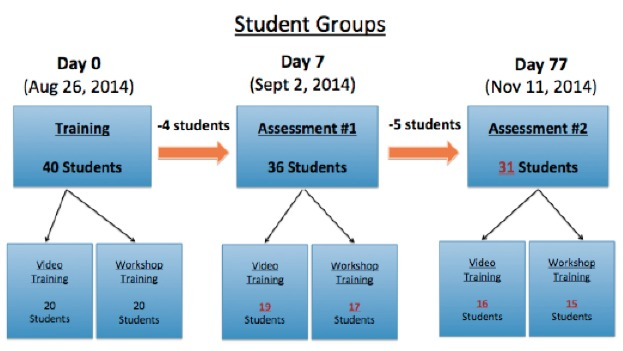
\includegraphics[width=0.8\linewidth]{Pictures/6_studyGroupsExample}
		\caption{Study groups example}
		\label{fig:6_studyGroups}
	\end{minipage}
\end{figure}

\subsubsection{Apparatus}
The setup can be seen in Figure \todo{[figure]}. The Kinect was attached on a tripod with a height of \todo{90 cm}. It was placed in front of the screen with the camera faced in the direction of the slackline. A beamer was \todo{mounted on the ceiling of the room} to project the interface on the screen in front of it. The slackline stood, like discussed in Section~\ref{5_1_technicalFeasibility}, directly in front of the Kinect. A marker was attached on the slackline to provide a starting point for the participant for getting up the line.
The set up for the human trainer group was the same, but without the screen. The video camera for recording was placed \todo{behind the slacker in a more diagonal way} to have her actions as well as the interface interaction recorded. The set up was not changed during the study to have the same condition for every participant.

\todo{[Figure]}

\subsection{Design}
\begin{comment}
2 between subject x 1 within subjects
2 (ISG vs HTG) x 1 (beginner)
ODER
3 dependent vs 2 independent variables
\end{comment}

\subsection{Procedure}
At first the participant was welcomed and then briefed about the idea as well as what she can expect from the study. Further an introduction about the training method in which she participates was given. After that she had to fill out a questionnaire for collecting demographic data and her prior experience with slacklining. The ISG had to answer one more question about the prior experience with interactive devices (e.g. Kinect, Wii, PlayStation Move, etc.).
%Therefore one can see if a person, which tends to have a better experience with the system during the study, relies on her prior experience with such devices. 
The physical activity level as well as the lateral preference was determined like stated above. Lastly she had to confirm a form consent.

\todo{pre-measurement eher allgemein halten und in 6.4.3 ausarbeiten oder testprozedere hier näher erläutern (attempts, wie lange maximal, marker an der slackline, etc.)?}

After that the participant had to stand on the ground as well as on a towel to obtain her general balance ability.
Further a pre-measurement was conducted to the slackline balance ability and the steps the participant is able to go on a slackline were measured for comparison.

The participant had to stay on a marked position, which gives the starting position of all exercises. Similarly a marker on the slackline visualises the starting position on the line for the participant. She had to execute all exercises either provided by the system or the trainer. These are divided into four levels with \todo{6, 4, 6, and 3 exercises}. Between each exercises the participant could take a break if desired.

After each accomplished exercise execution the participant was asked to rank the exercise regarding its difficulty. The ranking ranged from 1, very easy, to 5, very difficult. Therefore the assumption of the participant can be compared with the logged performance data. Further, it can be shown if the difficulty of the exercise set in each level is increasing and match the integrated exercise routine.

\todo{sollte die erklärung eher in \nameref{6_variables}?}

\todo{post-measurement eher allgemein halten und in 6.4.3 ausarbeiten oder testprozedere hier näher erläutern (attempts, wie lange maximal, marker an der slackline, etc.)?}

When finished with the training a post-measurement was conducted with the same procedure, like seen above in the pre-measurement.

Finally the participant had to answer questions a semi-structured interview to obtain her opinion on the general method and application scenarios for exactly this method with the slackline and other sport activities that could fit this method. Additionally the ISG were also interviewed about the user interface of the SLS and their experience with the interaction. The specific questions can be seen in \todo{Appendix}.
%for reviewing and validating performance parameters as well as to detect system failures.

\subsection{Independent and dependent variables}\label{6_variables}
The general balance ability of the participant was measured before training by how long she can stand on the ground and a towel. Comparing the results of the training method were conducted by standing on a slackline before and after the training. All measurements involves the left, right, and both feet and were counted in seconds. 

Furthermore, the participant had to made as many steps as she can on the slackline with the left and right foot as starting point. \todo{Hereby the steps were counted as comparison parameter}. Additionally the distance on the slackline was measured by dividing the device into five areas, each with a distance of 60 cm. Three attempts per side and method were executed and \todo{the best taken / the average calculated} to compare the results.

- \todo{exercise difficulty ranking, Interview questions?}

\todo{Dependent variables --> }
\begin{itemize}
\item Time stood on line with left, right, both feet
\item As many steps as possible on the line ( + distance with markers on the line) left, right feet
\item Accomplished exercises
\end{itemize}

\todo{Independent variables --> training method}

level?
\begin{itemize}
\item Interactive Slackline System
\item Human Trainer Group
\end{itemize}

\todo{Confounding variable}
\begin{itemize}
\item Experience with general balance training
\item Experience with slacklining
\item General physical activity
\end{itemize}

%A measurement of the participants' current balance performance was conducted before and after the training to compare the training results and learning progress.  This involves the measurement of how long the participant can stand on the slackline in seconds with her left, right, and with both feet. Further, how many steps were she able to walk on the slackline with the left or right foot for getting up the line. Three attempts per side and method were executed and \todo{the best taken / the average calculated} to compare the results.




